\documentclass[twoside]{article}
\usepackage[obeyspaces]{url}
\usepackage{natbib}
%\usepackage{chem}
\usepackage{color}
\usepackage{rotating} % loads graphicx
%\usepackage{longtable}
\usepackage{graphicx}
%\usepackage{verbatim}
%\usepackage{draftwatermark}\SetWatermarkScale{6}

\usepackage[nottoc]{tocbibind}
\settocbibname{References}          %%% Title of bibliography

\oddsidemargin-5mm
\evensidemargin-15mm
\topmargin-15mm
\textheight240mm
\textwidth180mm
\raggedbottom
\parindent0mm
\parskip1.0ex plus0.5ex minus0.5ex
\renewcommand{\arraystretch}{1}
\renewcommand{\topfraction}{0.95}
\renewcommand{\dbltopfraction}{0.95}
\renewcommand{\bottomfraction}{0.95}
\renewcommand{\floatpagefraction}{0.95}
\renewcommand{\dblfloatpagefraction}{0.95}
\renewcommand{\textfraction}{0.01}
\setcounter{topnumber}{3}
\setcounter{secnumdepth}{4}
\setcounter{tocdepth}{4}

\newcommand{\egcite}[1]{\citep[e.g.][]{#1}}
\newcommand{\etccite}[1]{\citep[and references therein]{#1}}
\newcommand{\hhline}{\noalign{\vspace{1mm}}\hline\noalign{\vspace{1mm}}}
\newcommand{\hhlines}{\noalign{\vspace{1mm}}\hline\hline\noalign{\vspace{1mm}}}
\newcommand{\kpproot}{{\sc root}}
\newcommand{\todo}[1]{{\uppercase{\bf ((#1))}}}

\def\mypageheader{A. Kerkweg et al.: TIMER User Manual}
\markboth{\mypageheader}{\mypageheader}
\pagestyle{myheadings}

\begin{document}

\thispagestyle{empty}
%\vspace*{2cm}
%\vspace*{-2cm}
\begin{center}
  {\Huge\bf MESSy TIMER User Manual}\\[3mm]
  {\huge\it for the MESSy TIMER submodel}\\[9mm]
  {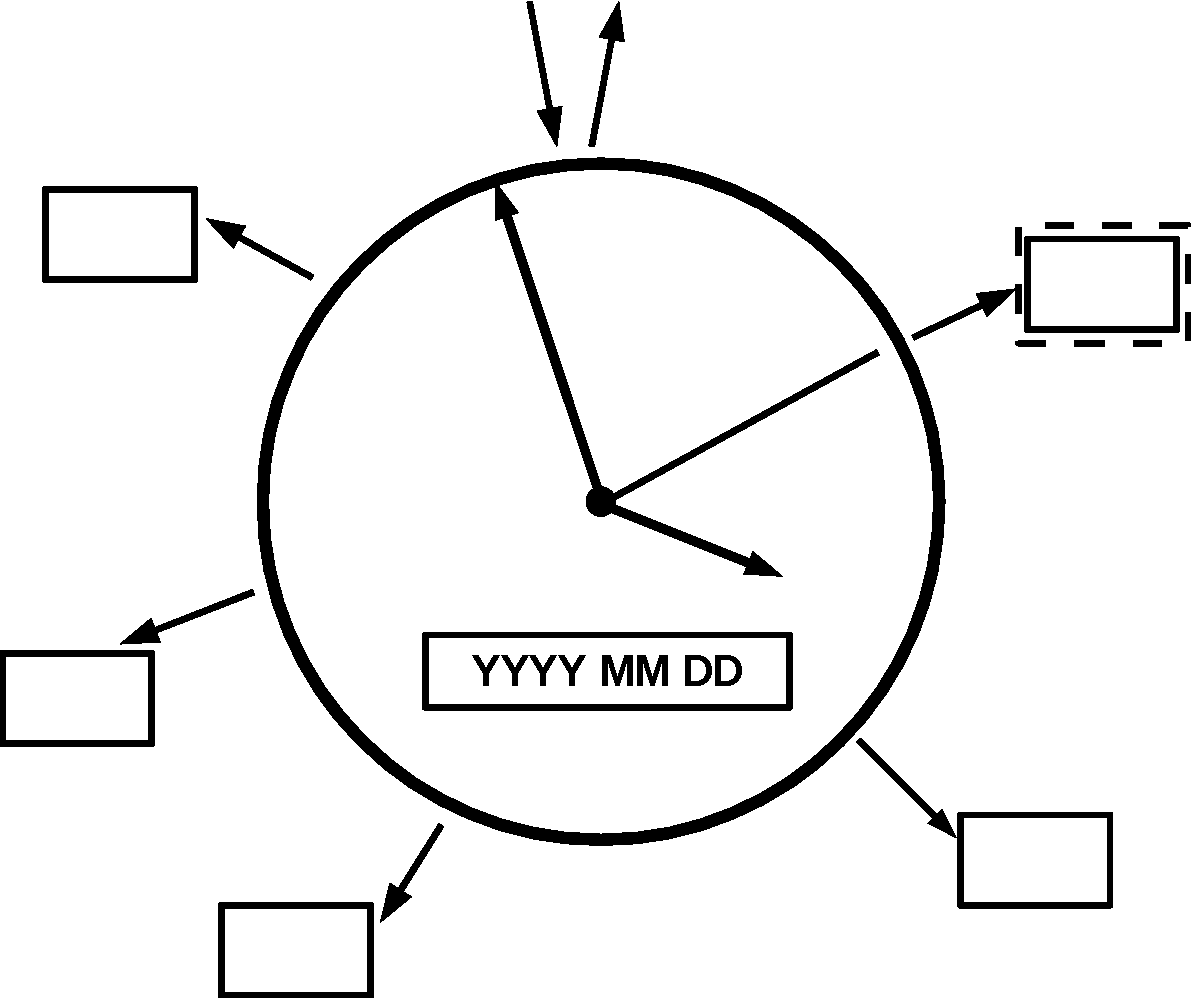
\includegraphics[width=0.7\textwidth]{timer_logo}}\\[9mm]
  {\huge\bf Astrid Kerkweg$^1$, Hella Riede$^2$ \& Patrick J\"ockel$^{2,3}$}\\[9mm]
  \small
  $^1$Institute for Atmospheric Physics,
  Johannes Gutenberg University Mainz
  55099 Mainz, Germany\\
  \url{kerkweg@uni-mainz.de}\\[3mm]

  $^2$
  Air Chemistry Department,
  Max-Planck Institute of Chemistry,
  PO Box 3060, 55020 Mainz, Germany\\

  $^3$ now at
  Deutsches Zentrum f\"{u}r Luft- und Raumfahrt,
  Institut f\"{u}r Physik der Atmosph\"{a}re,
  Oberpfaffenhofen, 82230 Wessling, Germany\\

\end{center}

\vfill

{\large This manual is part of the electronic supplement of our article
``Development Cycle 2 of the Modular Earth Submodel System (MESSy2)''
  in Geosci.\ Model\ Dev.\
  (2010), available at: \url{http://www.geoscientific-model-development.net}}

\begin{center}
  Date: \today
\end{center}

\newpage
\tableofcontents
\newpage

\newpage\twocolumn
\sloppy

%%%%%%%%%%%%%%%%%%%%%%%%%%%%%%%%%%%%%%%%%%%%%%%%%%%%%%%%%%%%%%%%%%%%%%%%%%%%%%
%% ###########################################################################
%%%%%%%%%%%%%%%%%%%%%%%%%%%%%%%%%%%%%%%%%%%%%%%%%%%%%%%%%%%%%%%%%%%%%%%%%%%%%%
\section{Introduction}
\label{sec:intro}
%%%%%%%%%%%%%%%%%%%%%%%%%%%%%%%%%%%%%%%%%%%%%%%%%%%%%%%%%%%%%%%%%%%%%%%%%%%%%%
%% ###########################################################################
%%%%%%%%%%%%%%%%%%%%%%%%%%%%%%%%%%%%%%%%%%%%%%%%%%%%%%%%%%%%%%%%%%%%%%%%%%%%%%
%
The MESSy \citep{442} generic submodel TIMER is partly based on the time
management routines of ECHAM5 \citep{478,479,480}. The TIMER provides the
timing information for the MESSy submodels and either replaces or mirrors the
timing information of the basemodel. In the first case, the initialisation of
the basemodel time information is overwritten by the TIMER namelist. In the
second case, the TIMER is initialised by the basemodel.
%
The submodel core layer (SMCL) of the TIMER consists of three Fortran95 modules:
%
\begin{itemize}
\item {\tt messy\_main\_timer.f90} provides 
      \begin{itemize}
      \item the basic type structure to store date and time information,
      \item the basic variables to store date and time information,
      \item tools (functions and subroutines) for date and time
            format conversions, time span calculations, etc.
      \end{itemize}
\item {\tt messy\_main\_timer\_manager.f90} provides the internal clock for
      the model simulation. It manages the time stepping and the date and time
      information during the simulation.
\item {\tt messy\_main\_timer\_event.f90} provides data types and routines to
      schedule processes at specific (regular) time intervals, e.g., to
      trigger regular output or input.
\end{itemize}
%
In addition the basemodel interface layer (BMIL) module
{\tt messy\_main\_timer\_bi.f90} provides the connection to the basemodel.

Figure~\ref{fig:timermodules} sketches the relationship between
the different Fortran95 modules of TIMER.
%
\begin{figure*}
  \centerline{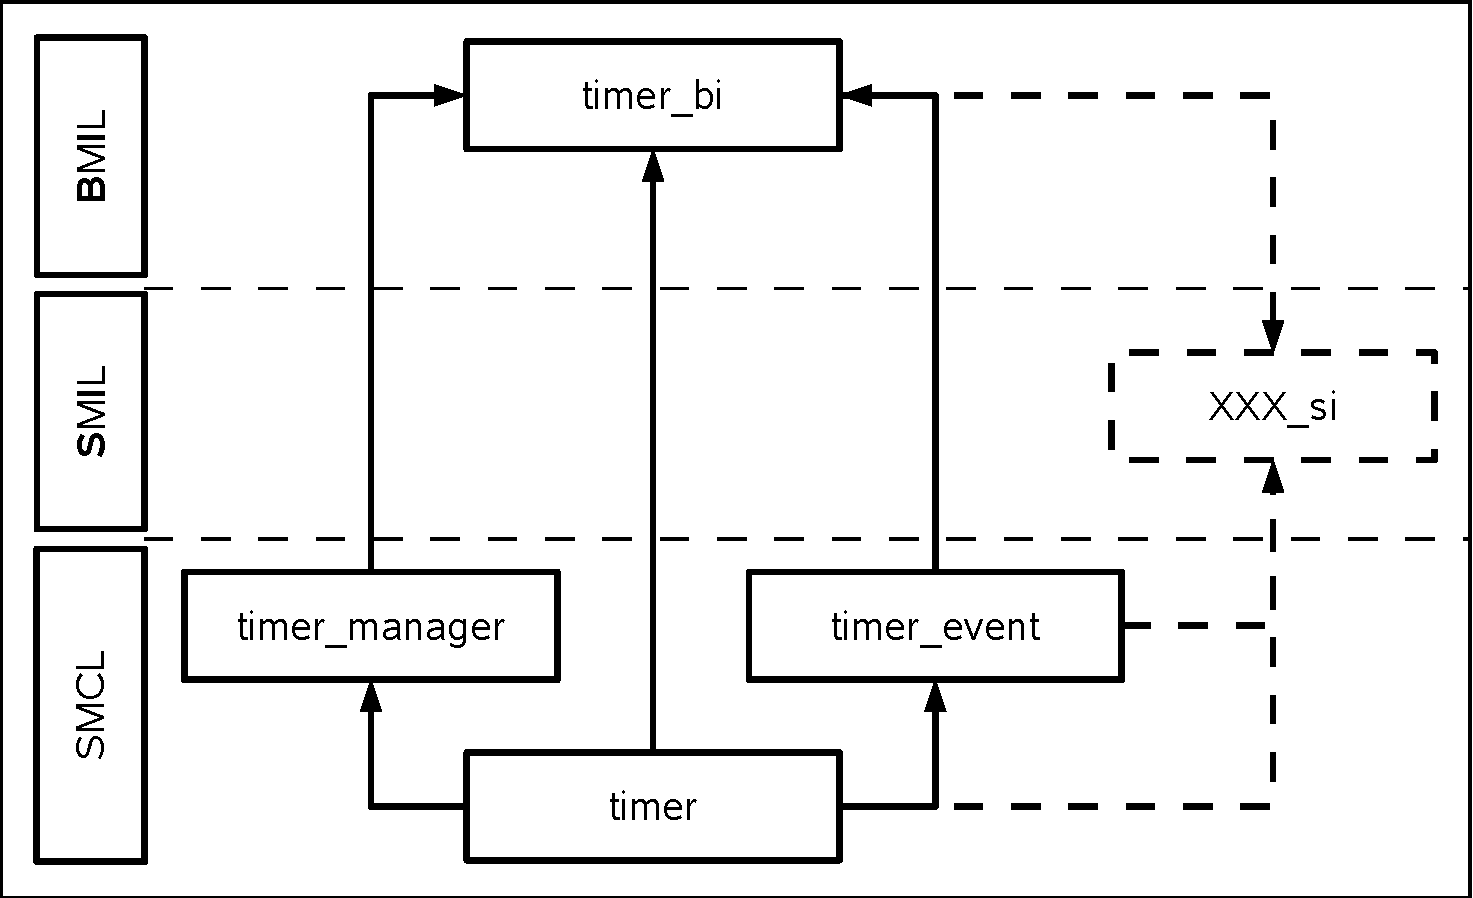
\includegraphics[width=0.7\textwidth]{timer_modules}}
  \caption[Relationship between TIMER modules] {Relationship between the
          various Fortran95 modules of TIMER: The boxes with horizonal
          text represent the different Fortran95 modules of TIMER, the
          corresponding filenames are {\tt messy\_main\_{\it TT.f90}}, where
          {\it TT} is the respective box text. The arrows indicate where the
          different modules are {\tt USE}d.  The dashed box with {\bf XXX}
          denotes an ordinary submodel, which makes use of the TIMER.  The
          different MESSy layers are indicated on the left side (SMCL:
          submodel core layer; SMIL: submodel interface layer; BMIL: basemodel
          interface layer) and by the module names (si = SMIL, bi = BMIL).  }
  \label{fig:timermodules}
\end{figure*}
%

%%%%%%%%%%%%%%%%%%%%%%%%%%%%%%%%%%%%%%%%%%%%%%%%%%%%%%%%%%%%%%%%%%%%%%%%%%%%%%
%% ###########################################################################
%%%%%%%%%%%%%%%%%%%%%%%%%%%%%%%%%%%%%%%%%%%%%%%%%%%%%%%%%%%%%%%%%%%%%%%%%%%%%%
\section{TIMER basics}
\label{sec:timer}
%%%%%%%%%%%%%%%%%%%%%%%%%%%%%%%%%%%%%%%%%%%%%%%%%%%%%%%%%%%%%%%%%%%%%%%%%%%%%%
%% ###########################################################################
%%%%%%%%%%%%%%%%%%%%%%%%%%%%%%%%%%%%%%%%%%%%%%%%%%%%%%%%%%%%%%%%%%%%%%%%%%%%%%

%%%%%%%%%%%%%%%%%%%%%%%%%%%%%%%%%%%%%%%%%%%%%%%%%%%%%%%%%%%%%%%%%%%%%%%%%%%%%%
\subsection{Representation of date and time}
\label{sec:types}
%%%%%%%%%%%%%%%%%%%%%%%%%%%%%%%%%%%%%%%%%%%%%%%%%%%%%%%%%%%%%%%%%%%%%%%%%%%%%%
There are two ways to represent a specific date and time within TIMER. 
%
Internally all dates are stored in a Fortran95 structure \verb|time_days| as
follows:
%
\begin{verbatim}
  TYPE, PUBLIC :: time_days 
     !
     ! relative calendar date 
     !               and time format
     !
     ! time_days [structure]
     !
     !    day    [integer] 
     !    (day in calendar,
     !      -2147483648 ... 2147483647
     !      approx. +/-5.8 Mio. years)
     !
     !    second [integer]  
     !     (seconds of day, 0,...,86399)
     !
     !PRIVATE
     LOGICAL :: init   = .FALSE.
     INTEGER :: day    = 0
     INTEGER :: second = 0
  END TYPE time_days
\end{verbatim}
%
This structure contains the two {\footnotesize INTEGER} components \verb|day| and
\verb|second| and in addition the {\footnotesize LOGICAL} component 
\verb|init|, which
indicates whether the date is already initialised (\verb|.TRUE.|) or
not (\verb|.FALSE.|).

The second representation of a date is the more descriptive form by
six {\footnotesize INTEGER} components for the year, month, day, hour,
minute and second,
respectively. For instance, the date ``10.11.2012 09:14:06'' 
is described by
YEAR=2012; MONTH=11; DAY=10; HOUR=9; MINUTE=14; SECOND=6.


%%%%%%%%%%%%%%%%%%%%%%%%%%%%%%%%%%%%%%%%%%%%%%%%%%%%%%%%%%%%%%%%%%%%%%%%%%%%%%
\subsection{Predefined variables}
\label{sec:predef}
%%%%%%%%%%%%%%%%%%%%%%%%%%%%%%%%%%%%%%%%%%%%%%%%%%%%%%%%%%%%%%%%%%%%%%%%%%%%%%
The TIMER provides predefined variables including some important date
variables, which are updated at the beginning of each simlation time step and
which are to be used by ordinary submodels. Usage of these variables prevents
the multiple re-calculation of the same information within one time step.
Additionally, some important switches (of {\footnotesize TYPE} {\footnotesize LOGICAL}) are
 defined, which are required for model run control.

%%%%%%%%%%%%%%%%%%%%%%%%%%%%%%%%%%%%%%%%

\subsubsection{Dates and times}
\label{sec:dates}
%
The predefined dates (of {\footnotesize TYPE} \verb|time_days|) provided by the TIMER
are:
%
\begin{itemize}
\item \verb|start_date|: the date and time of the simulation start,
\item \verb|stop_date|: the date and time at which the simulation finishes,
\item \verb|resume_date|: the date and time at which the simulation was
      resumed after a restart,
\item \verb|current_date|: the date and time of the current model time step,
\item \verb|previous_date|: the date and time of the previous model time step,
\item \verb|next_date|: the date and time of the next model time step.
\end{itemize}

%%%%%%%%%%%%%%%%%%%%%%%%%%%%%%%%%%%%%%%%

\subsubsection{{\footnotesize LOGICAL}s for model control}
\label{sec:logicals}
%
The predefined switches (of {\footnotesize TYPE} {\footnotesize LOGICAL}) provided by the TIMER
 are:
%
\begin{itemize}
\item \verb|lstart| is \verb|.TRUE.| during the initialisation phase and the
      very first time step of a simulation.
\item \verb|lresume| is \verb|.TRUE.| during the initialisation phase and the
      first time step after a model restart.  
\item \verb|lfirst_cycle| is \verb|.TRUE.| if \verb|lstart| or \verb|lresume|
      are \verb|.TRUE.|.
\item \verb|lbreak| is \verb|.TRUE.| during the last time step before a
      simulation will be interrupted (for later restart).
\item \verb|lstop| is \verb|.TRUE.| during the last time step before the end
      of the model simulation.
\item \verb|l_rerun| is \verb|.TRUE.| when restart files are to be written
  (see Sect. \ref{sec:restart}).
\item \verb|l_trigger_restart| is \verb|.TRUE.| when a restart is triggered
      by the generic submodel QTIMER.
\item \verb|labort| is set in the namelist. In case of \verb|.TRUE.|, the model 
      simulation will be finished after a break, even if \verb|stop_date| is 
      not reached. In other words, this switch prevents that after a model
      break the next job is submitted to the scheduler of the computer.
\item \verb|lforcedtime| indicates that the date and restart setting as defined
      in the namelist are overwritten by an external source. In TIMER itself
      the {\footnotesize LOGICAL} is used in \verb| main_timer_global_start| to
      prevent the setting of \verb|l_rerun| (as this also needs to be determined
      consistently by the external source).
\end{itemize}

%%%%%%%%%%%%%%%%%%%%%%%%%%%%%%%%%%%%%%%%

\subsubsection{Other variables}
\label{sec:others}
%
Some other variables are defined by TIMER as well:
%
\begin{itemize}
\item The {\footnotesize INTEGER} \verb|CAL_TYPE| defines the calendar type.
      Currently, two 
      calendar types are impemented:  The Julian calendar identified by the
      {\footnotesize INTEGER PARAMETER} \verb|CAL_JULIAN| and a 360 day per year
      calendar
      ({\footnotesize INTEGER PARAMETER} \verb|CAL_360D|). Note: the 360 day calendar option
      is implemented, but was NOT extensively tested.
\item \verb|INIT_STEP| is the position (step number) of the time manager (see
      Sect.~\ref{sec:time_manager}) at model simulation start.
\item \verb|delta_time| is the interval between two model time steps in
      seconds.
\item \verb|time_step_len| is the length of the integration time step, which
      depends on the integration scheme; e.g., a leap frog scheme uses a
      time step which is twice the interval of a model time step, whereas for
      a Runge-Kutta scheme the integration time step is equal to the time
      interval \verb|delta_time|.
\item \verb|YEAR,MONTH,DAY,HOUR,MINUTE,SECOND| contain the componentes of 
      \verb|current_date| as six {\footnotesize INTEGER} variables
      (Sect.~\ref{sec:dates}).
\item \verb|YEAR_START|, \verb|MONTH_START|, \verb|DAY_START|,
      \verb|HOUR_START|, \verb|MINUTE_START|, \verb|SECOND_START| contain the
      components of \verb|start_date| as six {\footnotesize INTEGER} variables.
\item \verb|YEAR_NEXT|, \verb|MONTH_NEXT|, \verb|DAY_NEXT|,
      \verb|HOUR_NEXT|, \verb|MINUTE_NEXT|, \verb|SECOND_NEXT| contain the
      components of \verb|next_date| as six {\footnotesize INTEGER} variables.
\item \verb|current_time_step| is of type {\footnotesize INTEGER} and equal to the position of 
      \verb|time_manager| (see Sect.~\ref{sec:time_manager}), which is the
      up-to-date count of the model time step.
\item \verb|CMONTHS| is a {\footnotesize CHARACTER ARRAY}
      of dimension 12, which contains 
      the three letter strings indicating the 12 months 
      ( \verb|'Jan'|, \verb|'Feb'|,
      \verb|'Mar'|, \verb|'Apr'|, \verb|'May'|, \verb|'Jun'|, \verb|'Jul'|, 
      \verb|'Aug'|, \verb|'Sep'|, \verb|'Oct|', \verb|'Nov'|, \verb|'Dec'|).
\item \verb|no_cycles| gives the number of how often restart files are written
      without interupting the simulation (see Sect. \ref{sec:restart}).
\item \verb|DAYOFYEAR| gives the number of the day in the current year, e.g.,
      \verb|1 Feb = 32|.
\end{itemize}

%%%%%%%%%%%%%%%%%%%%%%%%%%%%%%%%%%%%%%%%%%%%%%%%%%%%%%%%%%%%%%%%%%%%%%%%%%%%%%
\subsection{TIMER subroutines and functions}
%%%%%%%%%%%%%%%%%%%%%%%%%%%%%%%%%%%%%%%%%%%%%%%%%%%%%%%%%%%%%%%%%%%%%%%%%%%%%%
TIMER provides a lot of tools to handle dates and times and to simplify
time calculations in other submodels.

\subsubsection{TIMER routines called from the BML or BMIL}
%
A special class of subroutines are
those used to initialise the TIMER by the basemodel (from the basemodel
interface layer) or to initialise the basemodel time control by TIMER.
Their names start all with \verb|timer_|.
%
\begin{itemize}
\item \verb|timer_set_date| sets a date in {\footnotesize TYPE} \verb|time_days|
       format.
       The routine is fourfold overloaded. To define an arbitrary date the date
       to be set is parameter to the subroutine. For the six specific dates
      listed in Sect.~\ref{sec:dates}, alternatively a string can be specified
      (i.e., 'start', 'stop', 'resume', 'current', 'previous', 'next').
      
      Input for date definition are either 6 {\footnotesize INTEGER}s defining
      the
      date (year, month, day, hour, minute, second) or 2 
      {\footnotesize INTEGER}s giving the
      day and the second according to the {\footnotesize TYPE} \verb|time_days|
      format.

      In case of \verb|'start'| not only the \verb|start_date|
      will be set but also the {\footnotesize INTEGER}s \verb|YEAR_START|,
      \verb|MONTH_START|, \verb|DAY_START|, \verb|HOUR_START|,
      \verb|MINUTE_START|, \verb|SECOND_START| and \verb|JULIAN_DATE_START|.

      Examples:\\
      \verb|CALL timer_set_date(status, 'resume' &|
      \verb|, my_year, my_month, my_day &|
      \verb|, my_hour, my_minute, my_second)| \\ or \\
      \verb|CALL timer_set_date(status, 'resume' &|
      \verb|, date_day, date_second)| \\ or \\
      \verb|CALL timer_set_date(status, my_date &|
      \verb|, my_year, my_month, my_day &|
      \verb|, my_hour, my_minute, my_second)| \\ or \\
      \verb|CALL timer_set_date(status, my_date &|
      \verb|, date_day, date_second)|, \\ when \verb|my_date| is of
      {\footnotesize TYPE} \verb|time_days| and \verb|date_day| and 
      \verb|date_second| are of 
      {\footnotesize TYPE} \verb|time_days|.
 
\item \verb|timer_get_date| returns the six components of a date, namely year,
      month, day, hour, minute, second for an arbitrary date in
      \verb|time_days| format.  Alternatively, the six date components of the
      specific dates listed in section \ref{sec:dates} can be retrieved by
      specifying their name (i.e., 'start', 'stop', 'resume', 'current',
      'previous', 'next').  
      \\Examples: \\
      \verb|CALL timer_get_date(status, 'resume' &|
      \verb|, my_year, my_month, my_day &|
      \verb|, my_hour, my_minute, my_second)| \\ or \\
      \verb|CALL timer_get_date(status, my_date &|
      \verb|, my_year, my_month, my_day &|
      \verb|, my_hour, my_minute, my_second)|, \\ when \verb|my_date| is of
      {\footnotesize TYPE} \verb|time_days|.

\item \verb|timer_set_calendar| sets the calendar type of the TIMER.
\item \verb|timer_get_calendar| returns information about the calendar type of
      TIMER. 
\item \verb|timer_set_delta_time| sets the \verb|delta_time| of the TIMER 
      MANAGER (see Sect.~\ref{sec:time_manager}).
\item \verb|timer_get_delta_time| returns the \verb|delta_time| of the TIMER 
      MANAGER (see Sect.~\ref{sec:time_manager}).
\item \verb|timer_rewind_manager| rewinds the \verb|time_manager| 
      (see Sect.~\ref{sec:time_manager}).
\item \verb|timer_add_date| adds a time interval in seconds to a date
      specified by its six components and returns the new date in date
      components.
\item \verb|timer_set_lresume| sets the {\footnotesize LOGICAL} \verb|lresume|.
\item \verb|timer_get_lresume| returns the {\footnotesize LOGICAL} \verb|lresume| from the TIMER.
%\item \verb|write_date|: writes a date given in \verb|time_days| format into 
%      the logfile.
\item \verb|timer_set_time_step_len| sets the {\footnotesize INTEGER} \verb|time_step_len|.
\item \verb|timer_set_no_cycles|  sets the {\footnotesize INTEGER} \verb|no_cycles|.
\item \verb|timer_get_no_cycles| returns the {\footnotesize INTEGER} \verb|no_cycles| from TIMER.
\item \verb|timer_set_labort| sets the {\footnotesize LOGICAL} \verb|labort|.
\item \verb|timer_get_labort| returns the {\footnotesize LOGICAL} \verb|labort| from TIMER.
\item \verb|timer_set_rerun_event| defines the TIMER \verb|rerun_event| (see
 Sect. \ref{sec:restart}).
\item \verb|timer_get_rerun_event| provides the information about the TIMER
  \verb|rerun_event| (see Sect. \ref{sec:restart}) as given in the TIMER namelist
to the basemodel.
\item \verb|timer_message| provides an error message for a given error status.
\end{itemize}
%
Additionally, the FUNCTION \verb|timer_get_time_step| returns the position of 
the \verb|time_manager| (see Sect.~\ref{sec:time_manager}),
i.e., the model time step. 

%%%%%%%%%%%%%%%%%%%%%%%%%%%%%%%%%%%%%%%%

\subsubsection{Subroutines for date manipulations}
%
\begin{itemize}
\item \verb|date_set| sets a date in the \verb|time_days| format by
      specifiying the 2 {\footnotesize INTEGER}s \verb|day| and \verb|second| of the
      \verb|time_days| format.
\item \verb|date_set_components| sets a date in the \verb|time_days| format by
      specifying the 6 date components (year, month, day, hour, minute,
      second).
\item \verb|date_get| returns the 2 {\footnotesize INTEGER}s \verb|day| 
       and \verb|second| of a 
      date given as {\footnotesize TYPE}  \verb|time_days|.
\item \verb|date_get_components| returns the 6 date components of a date
      of {\footnotesize TYPE} \verb|time_days|.
\item \verb|add_date| add days and seconds to a date of {\footnotesize TYPE}
      \verb|time_days|.
\item \verb|copy_date| copies a date of  {\footnotesize TYPE} \verb|time_days| 
      into another
      variable of {\footnotesize TYPE} \verb|time_days|.
\item \verb|if_less| compares two dates of {\footnotesize TYPE} \verb|time_days|.
      A {\footnotesize LOGICAL}
      is set to \verb|.TRUE.|, if the first date is earlier than the second date.
\item \verb|if_equal| compares two dates of {\footnotesize TYPE} 
      \verb|time_days|. A {\footnotesize LOGICAL}
      is set to \verb|.TRUE.|, if both dates are equal.
\item \verb|is_init| returns the {\footnotesize LOGICAL} part of the 
       {\footnotesize TYPE} \verb|time_days| indicating if the date is
       initialised.
\item \verb|print_date| / \verb|write_date| write a date of {\footnotesize TYPE}
      \verb|time_days| to standard output. \verb|write_date| is the routine on
      BMIL level which calles the SMCL routines \verb|print_date| or
      \verb|print_date_components|.
\item \verb|print_date_components| writes the six date components of a date
       of {\footnotesize TYPE} \verb|time_days| to standard output.
\end{itemize}

%%%%%%%%%%%%%%%%%%%%%%%%%%%%%%%%%%%%%%%%%%%%%%%%%%%%%%%%%%%%%%%%%%%%%%%%%%%%%%
\subsection{Additional tools}
%%%%%%%%%%%%%%%%%%%%%%%%%%%%%%%%%%%%%%%%%%%%%%%%%%%%%%%%%%%%%%%%%%%%%%%%%%%%%%
%
\begin{itemize}
\item \verb|MonthLength| is a function to calculate the length of a month in
      days depending on the calendar type.
\item \verb|JulianMonthLength| is a function to calculate the length of a
      Julian month in days.
\item \verb|YearLength| is a function to calculate the length of a year in
      days depending on the calendar type.
\item \verb|JulianYearLength| is a function to calculate the length of a
      Julian year in days.
\item \verb|YearDay| is a function to calculate the number of a day in the
      current year depending on the calendar type.
\item \verb|julian_day| is a function to calculate the Julian day number
      for a Gregorian date (specified as year, month and day).
\item \verb|time_span_s| is a function to calculate the time difference in
      seconds between two Gregorian dates.
\item \verb|time_span_d| is a function to calculate the time difference in
      days between two Gregorian dates.
\item \verb|gregor2julian| converts a Gregorian date and time to the
      corresponding Julian date and fraction of the day.
\item \verb|julian2gregor| converts a Julian date and fraction of the day to
      the corresponding Gregorian date and time.
\item \verb|utc2lt| converts the time of day in UTC into local time for a
      given longitude.
\item \verb|eval_time_str| cracks common netcdf time string format (e.g.
           'seconds since 2000-01-01 00:00:00')  into date components.
\end{itemize}

Note: Only the non-Julian subroutines should be used to get proper
  results when applying the 360-days calendar.

%%%%%%%%%%%%%%%%%%%%%%%%%%%%%%%%%%%%%%%%%%%%%%%%%%%%%%%%%%%%%%%%%%%%%%%%%%%%%%
%% ###########################################################################
%%%%%%%%%%%%%%%%%%%%%%%%%%%%%%%%%%%%%%%%%%%%%%%%%%%%%%%%%%%%%%%%%%%%%%%%%%%%%%
\section{The TIME MANAGER}
\label{sec:time_manager}
%%%%%%%%%%%%%%%%%%%%%%%%%%%%%%%%%%%%%%%%%%%%%%%%%%%%%%%%%%%%%%%%%%%%%%%%%%%%%%
%% ###########################################################################
%%%%%%%%%%%%%%%%%%%%%%%%%%%%%%%%%%%%%%%%%%%%%%%%%%%%%%%%%%%%%%%%%%%%%%%%%%%%%%
%
The TIME MANAGER is the central unit for the time information of the model.
%
\subsection{Basic structure and subroutines}
%
The Fortran95 structure 
\verb|time_manager| contains all information to unambiguously
determine the time within a simulation:
%
\begin{verbatim}
  TYPE time_manager
     PRIVATE  ! no external access possible
     ! short description of the manager
     CHARACTER(STRLEN_MEDIUM) :: label = '' 
     ! initial date at pos=0
     TYPE (time_days)         :: start_date 
     ! manager state for access control
     LOGICAL  :: init         = .FALSE.  
     ! lock/unlock the manager
     LOGICAL  :: freeze       = .FALSE.  
     ! present step of the manager
     INTEGER  :: pos          = 0       
     ! time interval in seconds
     REAL(dp) :: delta_time   = 0._dp  
  END TYPE time_manager
\end{verbatim}
%
\verb|label| is the name of the \verb|time_manager|, and
\verb|start_date| is a Fortran95 structure (section \ref{sec:dates}),
which provides the date (day and time of day) of the simulation start.
%
The {\footnotesize LOGICAL} \verb|init| indicates whether the manager is already initialised, 
whereas \verb|freeze| indicates, whether the manager is locked, i.e., whether
the time manager is protected from further modifications.
%
As long as the {\footnotesize LOGICAL} \verb|freeze| is \verb|.FALSE.|, the contents of the
time manager might be changed. Freezing the time manager prevents it of
unintended changes.
%
Internally the manager counts steps. The respective counter is 
\verb|pos|; \verb|pos|$=0$ indicates the start of the simulation, i.e., at
\verb|start_date|. 
%
The length (in seconds) of one step is stored in \verb|delta_time|. For the
base model, this is usually the model time step length.
%
The manager is initialised with the fivefold overloaded
subroutine \verb|manager_init|. It comprises the possibilities to
%
\begin{itemize}
\item[a)] initialise the \verb|time_manager| by specifying the \verb|label|
          and the \verb|start_date| (\verb|manager_init_days|),
\item[b)] re-initialise the \verb|time_manager| by specifying a new
          \verb|start_date| provoking an adjustment of \verb|pos| 
          (\verb|manager_reinit_days|),
\item[c)] re-initialise the \verb|time_manager| by specifying a new time
          increment \verb|delta_time| provoking an adjustment of
          \verb|start_date| (\verb|manager_reinit_incr|),
\item[d)] re-position the \verb|time_manager| by specifying an offset to
          \verb|pos| (\verb|manager_step|),
\item[e)] lock/unlock the \verb|time_manager| by specifying the respective
          {\footnotesize LOGICAL} (\verb|.TRUE.| to lock the manager, \verb|.FALSE.| to unlock
          it) (\verb|manager_freeze|).
\end{itemize}
%
With the subroutine \verb|timer_rewind_manager| the \verb|time_manager| will be 
set to a new date. This can be achieved in two ways. 
%
First, the manager is rewind without changing the \verb|start_date|. This is
only possible, when the new date is later than the \verb|start_date|. In this
case the manager position \verb|pos| will be adjusted. 
%
The second method is to keep the position and the time interval, but to
change the \verb|start_date|.

The subroutine \verb|manager_print| prints the status of the manager to the
standard output.

The state of the \verb|time_manager| can be inquired using the subroutine 
\verb|manager_state|. 
Depending on the parameters, different information can be retrieved as 
listed in table \ref{tab:manager_state}.
%
\begin{table*}
\centering
\caption{Versions of suboutine {\tt|manager$\_$state|} \label{tab:manager_state}}
\begin{tabular}{llll}
INPUT & INPUT TYPE & OUTPUT TYPE & OUTPUT \\ \hline
position & {\footnotesize INTEGER}  & \verb|time_days| & corresponding date      \\
~~~-~~~  & ~~~~~~-         & \verb|time_days| & the current date    \\
a date   & \verb|time_days|& {\footnotesize INTEGER}   & nearst manager position \\
~~~-     & ~~~~~~-         & {\footnotesize REAL}      & \verb|delta_time|\\
~~~-     & ~~~~~~-         & {\footnotesize INTEGER}   & \verb|pos|\\
\end{tabular}
\end{table*}
%

\subsection{The heart beat of the TIME MANAGER}
%
The TIME MANAGER is initialised by the BMIL subroutine 
\verb|messy_timer_init_manager| which calls among others the SMCL 
\verb|manager_init|. 
\begin{verbatim}
CALL manager_init(BM_time,'base model time', 
                  start_date, timestep, m_text)
\end{verbatim} 
\verb|BM_time| is of {\footnotesize TYPE} \verb|time_manager| and thus the 
 {\footnotesize STRUCT} containing all
TIME MANAGER information. \verb|'base model time'| is the label of
 \verb|BM_time|.
\verb|start_date| is the date at which the manager starts, \verb|timestep| 
defines the  {\footnotesize STRUCT} element \verb|delta_time| of \verb|BM_time|
 and \verb|m_text| contains possible error output of the subroutine.

During the simulation the TIME MANAGER needs to be stepped forward at the 
very end of each model time 
step, thus starting the new one. This is done within the BMIL subroutine 
\verb|messy_timer_reset_time|. Here the position of the \verb|time_manager| is 
incremented by one. Afterwards, all dependent variables (e.g.\ dates and 
{\footnotesize LOGICAL}s) are updated accordingly.

%%%%%%%%%%%%%%%%%%%%%%%%%%%%%%%%%%%%%%%%%%%%%%%%%%%%%%%%%%%%%%%%%%%%%%%%%%%%%%
%% ###########################################################################
%%%%%%%%%%%%%%%%%%%%%%%%%%%%%%%%%%%%%%%%%%%%%%%%%%%%%%%%%%%%%%%%%%%%%%%%%%%%%%
\section{The EVENT MANAGER}
%%%%%%%%%%%%%%%%%%%%%%%%%%%%%%%%%%%%%%%%%%%%%%%%%%%%%%%%%%%%%%%%%%%%%%%%%%%%%%
%% ###########################################################################
%%%%%%%%%%%%%%%%%%%%%%%%%%%%%%%%%%%%%%%%%%%%%%%%%%%%%%%%%%%%%%%%%%%%%%%%%%%%%%
The EVENT MANAGER schedules events which are discrete in time, such
as the regular input and output of data, etc.

%%%%%%%%%%%%%%%%%%%%%%%%%%%%%%%%%%%%%%%%%%%%%%%%%%%%%%%%%%%%%%%%%%%%%%%%%%%%%%
\subsection{The definition of an event}
%%%%%%%%%%%%%%%%%%%%%%%%%%%%%%%%%%%%%%%%%%%%%%%%%%%%%%%%%%%%%%%%%%%%%%%%%%%%%%
An event is defined by the Fortran95 structure \verb|time_event|
%
\begin{verbatim}
  TYPE, PUBLIC :: time_event          
     ! hold all event relevant information
     PRIVATE
     ! event state for access control
     LOGICAL    :: init   = .FALSE.  
     ! event active true=on false=off
     LOGICAL    :: active = .FALSE.    
     ! increment between the action
     INTEGER    :: count  = 1          
     ! offset (seconds)
     INTEGER    :: offset = 0          
     ! adjustment interval in seconds
     REAL(dp)   :: delta      = 2.0_dp 
     REAL(dp)   :: half_delta = 1.0_dp
     ! descriptive label of the event
     CHARACTER(len=STRLEN_MEDIUM) ::  &
      label  = '' 
     !
     ! name of the basic units
     CHARACTER(len=STRLEN_SHORT)  ::  &
      unit   = TIME_INC_SECONDS 
     CHARACTER(len=STRLEN_SHORT)  ::  &
      adjust = TRIG_EXACT ! type of triggering
     !
     ! initial data for event
     TYPE (time_days)   ::     initial_date    
     ! without offset
     TYPE (time_days)   ::       cycle_date     
     ! previous trigger date
     TYPE (time_days)   :: previous_trigger  
     ! current trigger date
     TYPE (time_days)   ::  current_trigger  
     ! next trigger date
     TYPE (time_days)   ::     next_trigger  
     
  END TYPE time_event
\end{verbatim}
%
with the components as follows:
%
\begin{itemize}
\item \verb|initial_date| (of {\footnotesize TYPE} \verb|time_days|) is the date
       of the event initialisation.
\item \verb|init| is a {\footnotesize LOGICAL} indicating whether the event 
      is initialised.
\item \verb|active| is a {\footnotesize LOGICAL} indicating whether the event
      is active. An event can be defined / initialised but inactive. An inactive
      event will not trigger any action even if a trigger date is reached.
\item \verb|unit| is the unit in which the event is defined (either 'years',
      'months' ,'days', 'hours', 'minutes', 'seconds' or 'steps').
\item \verb|count| is an {\footnotesize INTEGER} increment between two dates at
      which the event is triggered; the increment is given in the unit
      specified by \verb|unit|.
\item \verb|delta| / \verb|half_delta| are intervals in seconds required for
      the internal calculation of the adjustment within the given interval.
\item \verb|label| is an unambiguous identifier (``name'') of the event which
      should be as descriptive as possible.
\item \verb|offset| is an {\footnotesize INTEGER} offset in seconds between the
      event defined \verb|count| and  \verb|unit| and  ``real'' event.  E.g.,
      the event is defined for each full hour, but it should always happen at 
      10 minutes past the full hour. In this case the offset would be 600
      (seconds). Note: the event defined by  \verb|count| and  \verb|unit| has
      to match full model time steps., i.e. count times the seonds equivalent to
      the unit must be a multiple of \verb|delta_time|. With \verb|offset| it is
      possible to schedule an event not exactly matching the time interval.  
      Note: it is not allowed to define an \verb|offset| for the \verb|unit|s
      'years' and  'months'.
\item \verb|adjust| is set to one of 'first', 'last' , 'exact' or 'off'.
      In case of 'off' the event is deactivated and will not be triggered
      at all.
      The effect of the other three strings depends on the chosen \verb|unit|.
      'exact' schedules the event in the time step where the trigger is located.
      'first' locates the event in the first time step after crossing the given
      date, whereas 'last' triggers the event in the last time step before the 
      actual event date. Examples:
      \begin{itemize}
        \item \verb|2,'hours','first',0| triggers the event exactly at
          \verb|2:00|, \verb|4:00|, \verb|6:00| etc..
        \item The 'exact' label triggers at the same time as the label 'first',
          if the \verb|offset| is zero.
        \item \verb|2,'hours','last',0| triggers one time step before 
          'first' 
          and 'exact' become true. In this example, assuming a time step of
          10 minutes, the event would be triggered 
          at \verb|1:50|, \verb|3:50|, \verb|5:50|, etc..
      \end{itemize}
      Note: The effect of the adjustment only comes into action when the 
      \verb|unit| is 'hours' or larger ('days', 'months','years'). 
      For 'steps',
      'seconds' and 'minutes' there is only an effect if the offset is neither a
      multiple of \verb|delta_time| nor zero. 
      Otherwise the events are triggered
      as if the adjustment would have been 'exact'.
      This leads to the effect,
      that \verb|120, 'minutes','last',0| triggers the event at
      different times
      as \verb|2,'hours','last',0|.

      Only if the offset causes the event to lie in between two model 
      time steps,
      the three \verb|adjust| strings apart from 'off' get a meaning for 
      all units smaller than 'hours'.
      'first' and 'last' adjust to the respective unit. I.e., 'first' rounds the
      seconds down to the current full count of \verb|unit|,
      whereas 'last' adjusts to the last count of \verb|unit|.
      E.g., if the model time step is 2 minutes:
\begin{itemize}
       \item The event is initialised via 
         \verb|10, 'minutes','adjust',300| i.e., the offset
         is 5 minutes (i.e. exact in the middle of two time steps).
         Then 'exact' and 'first' will cause the event to be triggered  at 
         6 minutes, 16 minutes and so on, whereas the 'last' adjustment results
         in a trigger after 4 minutes, 14 minutes etc.
       \item  The event is initialised via 
         \verb|10, 'minutes','adjust',290|. 
         Then 'first' and 'last' will cause the event to be triggered  at 
         6 minutes, 16 minutes and so on, whereas the 'exact' adjustment results
         in a trigger after 4 minutes, 14 minutes etc. 
       \item  The event is initialised via 
         \verb|10, 'minutes','adjust',240|. 
         Then 'first', 'exact' and 'last' will all cause the event to be 
         triggered after 4 minutes, 14 minutes etc. 
       \item  The event is initialised via 
         \verb|10, 'minutes','adjust', -290|. 
         Then 'first', 'exact' and 'last' will all cause the event to be 
         triggered  after 6 minutes, 16 minutes etc. 
\end{itemize}
\item \verb|previous_trigger| is the date in \verb|time_days| format at which
      the event was triggered last time.
\item \verb|current_trigger| is the date in \verb|time_days| format at which
      the event is triggered next (or now).
\item \verb|next_trigger| is the date in \verb|time_days| format at which the
      event will be triggered next after \verb|current_trigger|.
\item \verb|cycle_date| is the event date in \verb|time_days| format without 
      the offset. E.g. an event is defined for each full hour and an offset of 
      600 seconds. Thus the \verb|cycle_date| would be the full hour whereas the
      \verb|current_trigger| whould be five minutes past the full hour.
\end{itemize}
%

%%%%%%%%%%%%%%%%%%%%%%%%%%%%%%%%%%%%%%%%%%%%%%%%%%%%%%%%%%%%%%%%%%%%%%%%%%%%%%
\subsection{How to define an event?}
%%%%%%%%%%%%%%%%%%%%%%%%%%%%%%%%%%%%%%%%%%%%%%%%%%%%%%%%%%%%%%%%%%%%%%%%%%%%%%

An event is defined by four elements:
%
\begin{itemize}
\item \verb|counter| is an {\footnotesize INTEGER} defining the time interval
      (in units specified by \verb|unit|) at which the event is triggered.
\item \verb|unit| is the unit of the time interval for the trigger (either
      'years', 'months' ,'days', 'hours', 'minutes', 'seconds' or 'steps')
\item \verb|adjustment| is an adjustment within the time interval (either
      'first', 'last', 'exact' or 'off', see above).
\item \verb|offset| is an {\footnotesize INTEGER} offset in seconds between the
      event and the \verb|initial_date| of the event.
\end{itemize}
%
These four parameters are combined in the Fortran95 structure
\verb|io_time_event|:
%
\begin{verbatim}
  ! structures
  TYPE, PUBLIC :: io_time_event            
     ! external given event properties
     ! - No. of steps in given unit
     INTEGER     :: counter    = 0           
     ! - counter unit type
     CHARACTER(len=STRLEN_SHORT) :: &
       unit  = TIME_INC_SECONDS 
     ! - adjustment inside the unit
     CHARACTER(len=STRLEN_SHORT) :: &
       adjustment = TRIG_EXACT  
     ! - offset to initial date in seconds
     INTEGER     :: offset     = 0           
  END TYPE io_time_event
\end{verbatim}

With this, an event can be specified within a namelist, for instance
%
\begin{verbatim}
 EXAMPLE_EVENT  = 3,'hours','last',0  
\end{verbatim}
%
which determines \verb|counter|, \verb|unit|, \verb|adjustment|,
\verb|offset|. 
%
In this example the event will be triggered within every three hours
 (\verb|counter=3|,\verb|unit='hours'|). No offset is requested (0). The
\verb|adjustment| ='last' causes the event to be triggered in the time step 
before the 3 hours are reached.
Note: The offset is in seconds and not in the unit given by \verb|unit|.

These four variables must be defined (either by a namelist entry or
within the code) and a variable of {\footnotesize TYPE} \verb|io_time_event| must be 
initialized with these values. When the \verb|io_time_event| is initialised by 
namelist in a parallel environment, the information must be broadcasted from 
the namelist reading process to all other processes. This is achieved with
the subroutine \verb|p_bcast_event| ({\tt messy\_main\_timer\_bi.f90}).

The event itself is initialised by calling the BMIL subroutine 
\verb|timer_event_init|. Within this subroutine the event is tested (in
 subroutine \verb|event_eval|) for valid values and is defined afterwards
 by the SMCL subroutine \verb|event_init|.
The subroutine \verb|timer_event_init| requires as input:
%
\begin{itemize}
\item a variable of {\footnotesize TYPE} \verb|time_event|,
\item a variable of {\footnotesize TYPE} \verb|io_time_event| with the event
      settings,
\item the name of the event (i.e., the \verb|label|), and
\item a {\footnotesize CHARACTER} label (\verb|eval_date|) 
      indicating the evaluation date.
\end{itemize}
%
\verb|eval_date| indicates if the event will be evaluated with the present
date (i.e., the date of the current time step, \verb|EV_TLEV_PRES|), with the
\verb|next_date| (the date of the next time step, \verb|EV_TLEV_NEXT|) or with
the \verb|previous_date| (the date of the last time step, \verb|EV_TLEV_PREV|). 
%
The {\footnotesize CHARACTER PARAMETER}s \verb|EV_TLEV_PRES|, \verb|EV_TLEV_NEXT|
 and \verb|EV_TLEV_PREV|  are defined as \verb|'present'|, \verb|'next'| and
 \verb|'previous'|, respectively.
 Note: The \verb|eval_date| must always correspond to the 
date with which the event is tested later on (call of  \verb|event_state|).
If \verb|event_state| is called with  \verb|current_date|  \verb|eval_date| must
be \verb|EV_TLEV_PRES| for \verb|next_date| it must be \verb|EV_TLEV_NEXT| and 
if \verb|event_state| is called with  \verb|previous_date| the \verb|eval_date|
should be  \verb|EV_TLEV_PREV|.

%%%%%%%%%%%%%%%%%%%%%%%%%%%%%%%%%%%%%%%%%%%%%%%%%%%%%%%%%%%%%%%%%%%%%%%%%%%%%%
\subsection{How to inquire an event?}
%%%%%%%%%%%%%%%%%%%%%%%%%%%%%%%%%%%%%%%%%%%%%%%%%%%%%%%%%%%%%%%%%%%%%%%%%%%%%%
For each of the state variables defined within the Fortran95 structure
\verb|time_event| a function exists providing the respective information:
%
\begin{itemize}
\item \verb|event_is_init|
\item \verb|event_is_active|
\item \verb|event_count|
\item \verb|event_offset|
\item \verb|event_delta|
\item \verb|event_half_delta|
\item \verb|event_label|
\item \verb|event_adjust|
\item \verb|event_unit|
\end{itemize}

In addition, subroutines are defined to provide the respecitive dates:
%
\begin{itemize}
\item \verb|event_initial_date|
\item \verb|event_cycle_date|
\item \verb|event_previous_date|
\item \verb|event_current_date|
\item \verb|event_next_date|
\end{itemize}

Depending on the input, the overloaded subroutine \verb|event_state| provides 
%
\begin{itemize}
\item the interval between the previous and the current trigger as number of 
      steps of unit \verb|unit|,
\item the time interval between the previous and the current trigger as 
      number of seconds, or
\item the time interval between the current and the next trigger as 
      number of seconds.
\item a {\footnotesize LOGICAL} which is \verb|.TRUE.| if the event should be triggered this
      time step.
\end{itemize}

%%%%%%%%%%%%%%%%%%%%%%%%%%%%%%%%%%%%%%%%%%%%%%%%%%%%%%%%%%%%%%%%%%%%%%%%%%%%%%
%% ###########################################################################
%%%%%%%%%%%%%%%%%%%%%%%%%%%%%%%%%%%%%%%%%%%%%%%%%%%%%%%%%%%%%%%%%%%%%%%%%%%%%%
\subsection{The restart event\label{sec:restart}}
%%%%%%%%%%%%%%%%%%%%%%%%%%%%%%%%%%%%%%%%%%%%%%%%%%%%%%%%%%%%%%%%%%%%%%%%%%%%%%
%% ###########################################################################
%%%%%%%%%%%%%%%%%%%%%%%%%%%%%%%%%%%%%%%%%%%%%%%%%%%%%%%%%%%%%%%%%%%%%%%%%%%%%%
A specific event is the restart (or rerun) event, a pre-defined
\verb|time_event| labeled ``rerun\_event''.

If this event is triggered, the status of the model is dumped with full
precision to restart files and - depending on the number of cycles -
the simulation is interrupted. The restart files are then used to continue the
model simulation.

Note: the {\footnotesize LOGICAL}s \verb|l_rerun| and \verb|lbreak| 
(see Sect. \ref{sec:logicals})  and the variable \verb|no_cycles| 
(see Sect. \ref{sec:others}) gain together a rather complex meaning: 
\verb|l_rerun| is the result of the function
 \verb|event_state|. If \verb|.TRUE.| restart files will be written. This itself
does not imply any consequences for the continuation of the model simulation.
But, each time  restart files are written the counter of \verb|cycles| will be
increased by 1. When the number of maximal cycles (\verb|no_cycles|) given in 
 the namelist is reached, the {\footnotesize LOGICAL} \verb|lbreak| will be set
 \verb|.TRUE.| and as consequence the simulation will be interupted.

There are two ways of defining the \verb|rerun_event|. Either it can be 
initialised from the settings of the basemodel or it is defined within the timer
namelist. The second is the more apropriate way, but to keep the full 
functionality of the basemodel it might be desirable to use the timing of the
basemodel. If the restart event is determined by the basemodel, the subroutine
\verb|timer_set_rerun_event| must be called.
 The information required from the basemodel are:
The four components of the \verb|io_time_event| and the string indicating, if
the evaluation of the event will be performed with the present or the next
date.
For setting the restart event via namelist see Section \ref{sec:namelist}.

%%%%%%%%%%%%%%%%%%%%%%%%%%%%%%%%%%%%%%%%%%%%%%%%%%%%%%%%%%%%%%%%%%%%%%%%%%%%%%
\subsection{Subroutines used internally} 
%%%%%%%%%%%%%%%%%%%%%%%%%%%%%%%%%%%%%%%%%%%%%%%%%%%%%%%%%%%%%%%%%%%%%%%%%%%%%%
%
\begin{itemize}
\item \verb|event_init| is called by \verb|timer_event_init|. Within this
      subroutine the variables contained in the Fortran95 structure
      \verb|time_event| are tested for consistency and the event is
      initialised.
\item \verb|event_reinit| re-initialises an event in the way that the current
      and the next trigger date are reset to the date given as parameter.
      This works only for dates later than the current date.
\item \verb|print_event_name| writes the event name to standard output.
\item \verb|convert_steps2unit| converts the counter which is defined in steps
      into a counter for the new unit \verb|unit|.
\item \verb|get_next_trigger| resets the event trigger after an
      event was triggered. This subroutine contains the subroutine 
      \verb|get_next_date|. 
\item \verb|adjust_date| adjusts the interval to the date  according to the
      event element \verb|adjust|.
\item \verb|event_print| prints the triggers and the initialisation information
      of an event.
\end{itemize}

%%%%%%%%%%%%%%%%%%%%%%%%%%%%%%%%%%%%%%%%%%%%%%%%%%%%%%%%%%%%%%%%%%%%%%%%%%%%%%
%% ###########################################################################
%%%%%%%%%%%%%%%%%%%%%%%%%%%%%%%%%%%%%%%%%%%%%%%%%%%%%%%%%%%%%%%%%%%%%%%%%%%%%%
\section{The TIMER namelist}
\label{sec:namelist}
%%%%%%%%%%%%%%%%%%%%%%%%%%%%%%%%%%%%%%%%%%%%%%%%%%%%%%%%%%%%%%%%%%%%%%%%%%%%%%
%% ###########################################################################
%%%%%%%%%%%%%%%%%%%%%%%%%%%%%%%%%%%%%%%%%%%%%%%%%%%%%%%%%%%%%%%%%%%%%%%%%%%%%%
The time control of a model simulation is defined in the CPL namelist of TIMER
in \verb|timer.nml| (see Fig. \ref{nml}).
%
\begin{figure*}
\small
\begin{verbatim}
! -*- f90 -*-
&CPL
CAL_TYPE    = 0,  !# 0: julian calendar
                  !# 1: 360 day year
!
!# automatically set by run-script; do not change
MODEL_START = $START_YEAR,$START_MONTH,$START_DAY,$START_HOUR,0,0,
MODEL_STOP  = $STOP_YEAR, $STOP_MONTH, $STOP_DAY, $STOP_HOUR,0,0,
lresume     = $ESH_LRESUME,
!
!# trigger restart at this time interval
IO_RERUN_EV = 1,'months','last',0,
no_cylces   = 2,                     ! restart cycles without break
LABORT      = F,                     ! abort after first cycle in any case
! 
!# set model time step here; if undefined it is automatically set by the
!# basemodel (ECHAM5 only!)
delta_time  = 600,                ! in seconds
!
/

\end{verbatim}
\caption{The CPL namelist of TIMER in \tt{timer.nml} \label{nml}}
\end{figure*}
%

\begin{itemize}
\item \verb|CAL_TYPE| is an {\footnotesize INTEGER} determining the applied
      calendar.
      It can be either the Julian calendar (0), or a climatological calendar
      using a 360 day year (1). NOTE: the 360 day year calendar was implemented
      but never tested thoroughly. Be careful in using option 1. 
\item \verb|MODEL_START| is an {\footnotesize INTEGER} array containing the 6 date
      components of the start date. Within MESSy they will be usually set in
      the run-script and exportet to the namelist via the shell variables
      \verb|$START_YEAR|, \verb|$START_MONTH|, \verb|$START_DAY|,
      \verb|$START_HOUR|.
\item \verb|MODEL_STOP| is an {\footnotesize INTEGER} array containing the 6 date
      components of the stop date. Within MESSy they will be usually set in
      the run-script and exportet to the namelist via the shell variables
      \verb|$STOP_YEAR|, \verb|$STOP_MONTH|, \verb|$STOP_DAY| and
      \verb|$STOP_HOUR|.
\item \verb|lresume| is \verb|.TRUE.| in case of a model restart. It is also
      set automatically by the run-script.
\item \verb|IO_RERUN_EV| determines the restart event. It
      is of the {\footnotesize TYPE} \verb|io_rerun_event|.
\item \verb|LABORT| prevents (if .TRUE.) that after a model break the next job
      is submitted to the scheduler of the computer.
\item \verb|no_cycles| defines the number of rerun cycles after which the model
      simulation is interrupted (see Sect. \ref{sec:others}.
\item \verb|delta_time| is the model time step used in the simulation.
\end{itemize}

%%%%%%%%%%%%%%%%%%%%%%%%%%%%%%%%%%%%%%%%%%%%%%%%%%%%%%%%%%%%%%%%%%%%%%%%%%%%%%
%% ###########################################################################
%%%%%%%%%%%%%%%%%%%%%%%%%%%%%%%%%%%%%%%%%%%%%%%%%%%%%%%%%%%%%%%%%%%%%%%%%%%%%%
\section{The TIMER BMIL ROUTINES}
\label{sec:BMIL}
Within the timeflow of a model simulation the following TIMER BMIL routines
must be called to operate the TIMER:

\begin{itemize}
\item \verb|main_timer_setup(flag)| should be called as early as possible within 
 the initialisation phase. For flag=1 the TIMER namelist is
 read via \verb|main_timer_read_nml_cpl| and broadcasted to all CPUs. 
 Furthermore the {\footnotesize LOGICAL} \verb|lstart| and \verb|lfirst_cycle| are set.
 For flag=2  \verb|start_date| and \verb|stop_date| are set according to the
 namelist (if not yet initialised) and the \verb|io_rerun_event| will be
 defined from the namelist and broadcasted. Additionally the first TIME MANAGER
 initialisation takes part here.
 
 Note: the separation of \verb|main_timer_setup| into two
 parts is required to enable the TIMER to be initialised by the basemodel
 instead of the timer namelist.  
\item \verb|main_timer_initialize| is called from \verb|messy_initialize|. First,
 within the internal subroutine  \verb|init_BM_time| the TIMER variables 
\verb|previous_date|, \verb|next_date|, \verb|current_date|, \verb|start_date|
 and \verb|time_step_len| are initialised or updated, respectively.
Additionally, the variable \verb|current_time_step| and the date components
for the  \verb|start_date| \verb|YEAR_START|, \verb|MONTH_START|,
\verb|DAY_START|, \verb|HOUR_START|, \verb|MINUTE_START|, \verb|SECOND_START| are
initialised. Only in case of a start of a model simulation
 (lstart = \verb|.TRUE.|, i.e.,~no restart), the date components of the
  \verb|current_date| ( \verb|YEAR|, \verb|MONTH|, \verb|DAY|, \verb|HOUR|, 
\verb|MINUTE|, \verb|SECOND|) are set in this subroutine.
  Finally, the restart event is defined by the subroutine 
  \verb|timer_event_init|.

\item \verb|main_timer_global_start|
  First the \verb|rerun_event| is evaluated and the {\footnotesize LOGICAL} \verb|l_rerun| is
  set. Secondly, the \verb|next_date| is evaluated according to the
  \verb|stop_date|. When the \verb|stop_date| will be reached in the following
  time step, the {\footnotesize LOGICAL}  \verb|lstop| is set \verb|.TRUE.|. In this case
  the {\footnotesize LOGICAL}s  \verb|l_rerun| and  \verb|L_TRIGGER_RESTART| will also be set
  \verb|.TRUE.|. Thirdly, \verb|lbreak| will be set dependent on \verb|l_rerun|,
  \verb|no_cycles| and  \verb|L_TRIGGER_RESTART|. At the end the date components
  \verb|YEAR|, \verb|MONTH|, \verb|DAY|, \verb|HOUR|, 
  \verb|MINUTE|, \verb|SECOND| and \verb|YEAR_NEXT|, \verb|MONTH_NEXT|,
  \verb|DAY_NEXT|, \verb|HOUR_NEXT|, \verb|MINUTE_NEXT|, \verb|SECOND_NEXT|
  are reset.
\item \verb|messy_timer_reset_time|
  The position of the TIME MANAGER is incremented by one and the dates 
  (\verb|previous_date|, \verb|next_date|, \verb|current_date|) 
  updated accordingly. Additionally the {\footnotesize LOGICAL}s  \verb|lstart|,
     \verb|lresume| and \verb|lfirst_cycle| are set to \verb|.FALSE.|.
\end{itemize}

%%%%%%%%%%%%%%%%%%%%%%%%%%%%%%%%%%%%%%%%%%%%%%%%%%%%%%%%%%%%%%%%%%%%%%%%%%%%%%
%% ###########################################################################
%%%%%%%%%%%%%%%%%%%%%%%%%%%%%%%%%%%%%%%%%%%%%%%%%%%%%%%%%%%%%%%%%%%%%%%%%%%%%%
%%%%%%%%%%%%%%%%%%%%%%%%%%%%%%%%%%%%%%%%%%%%%%%%%%%%%%%%%%%%%%%%%%%%%%%%%%%%%%
\bibliographystyle{copernicus} % bst file
\bibliography{main_timer}  % bib file
%%%%%%%%%%%%%%%%%%%%%%%%%%%%%%%%%%%%%%%%%%%%%%%%%%%%%%%%%%%%%%%%%%%%%%%%%%%%%%
\end{document}


